\documentclass[border=10pt]{standalone}
\usepackage{tikz}
\usepackage{amsmath}
\usepackage{amssymb}
\usetikzlibrary{shapes.geometric, arrows.meta, positioning, fit, backgrounds}

\begin{document}
	
	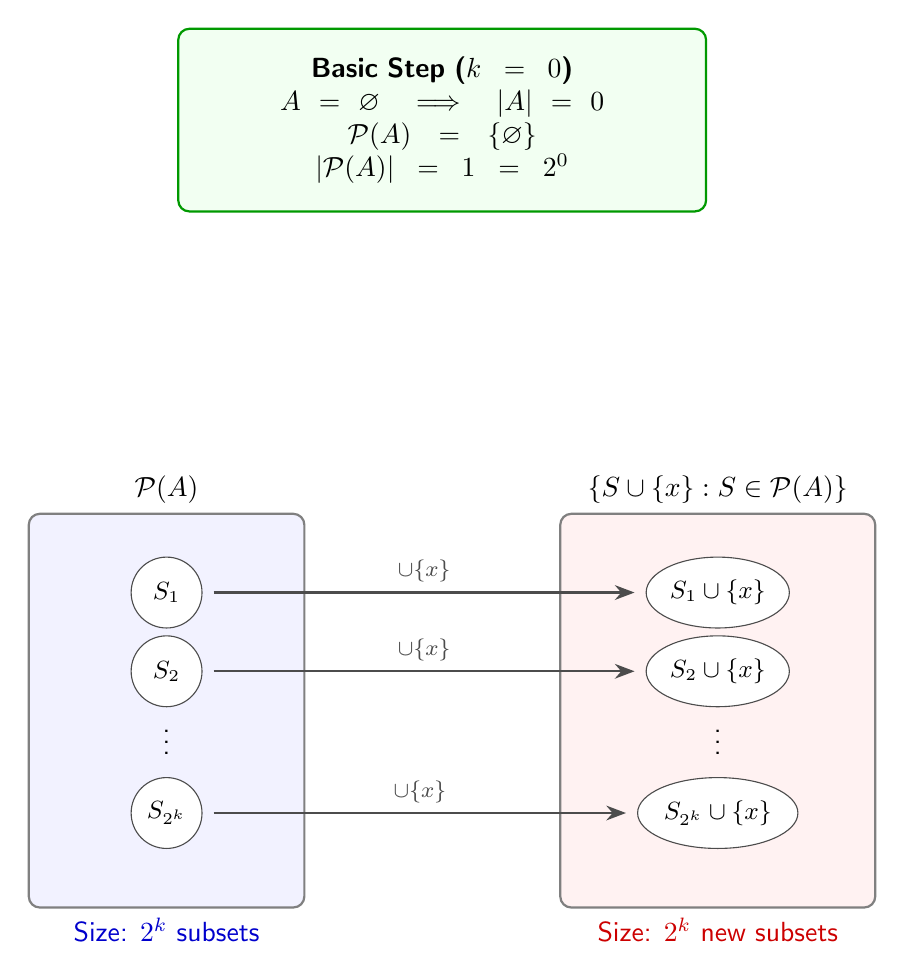
\begin{tikzpicture}[
		font=\sffamily,
		setbox/.style={draw=black!50, thick, rounded corners, fill=blue!5, minimum width=3.5cm, minimum height=5cm, align=center},
		newsetbox/.style={draw=black!50, thick, rounded corners, fill=red!5, minimum width=4cm, minimum height=5cm, align=center},
		element/.style={draw=black!70, circle, fill=white, inner sep=1pt, minimum size=0.9cm, font=\small},
		arrow/.style={-{Stealth[length=2.5mm]}, thick, draw=black!70, shorten >= 4pt, shorten <= 4pt}
		]
		
		% ==========================================
		% BASIC STEP
		% ==========================================
		\node[draw=green!60!black, thick, rounded corners, fill=green!5, text width=6cm, align=center, inner sep=10pt] (base) at (3.5, 7) {
			\textbf{Basic Step ($k=0$)}\\
			$A = \varnothing \implies |A| = 0$ \\
			$\mathcal{P}(A) = \{\varnothing\}$ \\
			$|\mathcal{P}(A)| = 1 = 2^0$
		};
		
		% ==========================================
%		% INDUCTIVE STEP BOUNDING BOX
%		% ==========================================
%		\draw[draw=black!30, dashed, rounded corners, fill=gray!2] (-2.5, -4.5) rectangle (9.5, 5);
%		\node[text=black!80, font=\large\bfseries] at (3.5, 4.3) {Inductive Step: Constructing $\mathcal{P}(A')$};
%		\node[text=black!80] at (3.5, 3.6) {Let $A' = A \cup \{x\}$, where $x \notin A$ and $|A| = k$};
		
		% ==========================================
		% P(A) BOX (Left Side)
		% ==========================================
		\node[setbox] (PA) at (0, -0.5) {};
		\node[anchor=south, font=\bfseries] at (PA.north) {$\mathcal{P}(A)$};
		\node[anchor=north, text=blue!80!black] at (PA.south) {Size: $2^k$ subsets};
		
		% Elements inside P(A)
		\node[element] (s1) at (0, 1) {$S_1$};
		\node[element] (s2) at (0, 0) {$S_2$};
		\node at (0, -0.8) {$\vdots$};
		\node[element] (sn) at (0, -1.8) {$S_{2^k}$};
		
		% ==========================================
		% P(A') NEW ELEMENTS BOX (Right Side)
		% ==========================================
		\node[newsetbox] (PAx) at (7, -0.5) {};
		\node[anchor=south, font=\bfseries] at (PAx.north) {$\{S \cup \{x\} : S \in \mathcal{P}(A)\}$};
		\node[anchor=north, text=red!80!black] at (PAx.south) {Size: $2^k$ new subsets};
		
		% Elements inside New Sets Box
		\node[element, ellipse] (s1x) at (7, 1) {$S_1 \cup \{x\}$};
		\node[element, ellipse] (s2x) at (7, 0) {$S_2 \cup \{x\}$};
		\node at (7, -0.8) {$\vdots$};
		\node[element, ellipse] (snx) at (7, -1.8) {$S_{2^k} \cup \{x\}$};
		
		% ==========================================
		% ARROWS (Bijection mapping)
		% ==========================================
		\draw[arrow] (s1) -- node[above, font=\footnotesize, text=black!70] {$\cup \{x\}$} (s1x);
		\draw[arrow] (s2) -- node[above, font=\footnotesize, text=black!70] {$\cup \{x\}$} (s2x);
		\draw[arrow] (sn) -- node[above, font=\footnotesize, text=black!70] {$\cup \{x\}$} (snx);
		
%		% ==========================================
%		% CONCLUSION EQUATION
%		% ==========================================
%		\node[align=center, fill=white, draw=black!20, rounded corners, inner sep=8pt] at (3.5, -3.5) {
%			$\mathcal{P}(A') = \mathcal{P}(A) \cup \{S \cup \{x\} : S \in \mathcal{P}(A)\}$ \\[1ex]
%			$|\mathcal{P}(A')| = \underbrace{|\mathcal{P}(A)|}_{2^k} + \underbrace{|\{S \cup \{x\} : S \in \mathcal{P}(A)\}|}_{2^k} = 2^{k+1}$
%		};
		
	\end{tikzpicture}
	
\end{document}